\documentclass[12pt]{article}

\usepackage{sbc-template}
\usepackage{graphicx,url}
\usepackage[english]{babel}
\usepackage[T1]{fontenc}
\usepackage[utf8]{inputenc}
\usepackage{multicol}
\usepackage{multirow}
\usepackage{amsmath,amssymb,amsfonts}
\usepackage{textcomp}
\usepackage{url}
\usepackage{enumerate}
\usepackage{verbatim}
\usepackage[table,xcdraw]{xcolor}
\usepackage[shortlabels]{enumitem}
\usepackage{fancyhdr}
\usepackage{sbgames}
\usepackage{booktabs}
\usepackage{tikz}
\usetikzlibrary{positioning,arrows.meta,shapes.geometric,calc,shadows}

% C4 Model colors and styles
\definecolor{c4person}{RGB}{8, 63, 115}
\definecolor{c4system}{RGB}{17, 119, 210}
\definecolor{c4external}{RGB}{153, 153, 153}
\definecolor{c4container}{RGB}{67, 131, 191}
\definecolor{c4database}{RGB}{67, 131, 191}

\tikzset{
    c4base/.style={
        rectangle, rounded corners=2pt, draw=white, thick,
        text=white, align=center, font=\sffamily\bfseries,
        drop shadow={opacity=0.2}
    },
    c4person/.style={
        c4base, fill=c4person, minimum width=2.8cm, minimum height=1.3cm
    },
    c4system/.style={
        c4base, fill=c4system, minimum width=3.6cm, minimum height=1.6cm
    },
    c4external/.style={
        c4base, fill=c4external, minimum width=3.0cm, minimum height=1.4cm
    },
    c4container/.style={
        c4base, fill=c4container, minimum width=3.1cm, minimum height=1.3cm
    },
    c4db/.style={
        cylinder, cylinder uses custom fill, cylinder body fill=c4database,
        cylinder end fill=c4database!80, shape border rotate=90,
        draw=white, thick, text=white, align=center, font=\sffamily\bfseries,
        minimum width=2.2cm, minimum height=1.6cm, drop shadow={opacity=0.2}
    },
    c4rel/.style={
        -{Stealth[length=2.5mm]}, thick, draw=gray!80, font=\sffamily\footnotesize,
        text=black!80, align=center
    }
}

\tolerance=1
\emergencystretch=\maxdimen
\hyphenpenalty=10000
\hbadness=10000

\sloppy


\trilha{Informe a Trilha} %Preencha com: Artes \& Design | Computação | Cultura | Saúde | Indústria | Educação | Tutoriais | MAGICA | WGP-Jogos
\local{Cidade/UF} % Exemplo: Manaus/AM
\ano{20XX} % Exemplo: 2024
\edicao{Edição (Romano)} %Exemplo: XXIII

\title{Evaluating Interactive LLM-Based Systems: A Reproducible Protocol for Narrative Coherence and State Consistency}

\author{[OMITTED FOR ANONYMOUS REVIEW]}

\address{[OMITTED FOR ANONYMOUS REVIEW]
  \email{[OMITTED FOR ANONYMOUS REVIEW]}
}

\begin{document}

\maketitle

\thispagestyle{plain}

\begin{abstract}
Evaluating interactive Large Language Model (LLM)-based systems, such as Game Masters in role-playing games (RPGs), remains a challenging problem due to the multi-turn, stateful, and subjective nature of these interactions. This paper presents a reproducible evaluation protocol for interactive LLM-based systems based on LLM-as-a-judge and operating over structured gameplay logs. The protocol is organized around six explicit functional requirements (multi-turn evaluation, state awareness, reproducibility, model-agnostic operation, metric-based assessment, and scalability) and defines a metric-driven pipeline that captures narrative quality, action-to-narration coherence, and state consistency. Unlike prior approaches focused on static or controlled benchmarks, the protocol evaluates full gameplay sessions, enabling analysis of long-term behavior and state evolution, and supports local LLM deployment for reproducibility. The protocol effectively differentiates system performance across four open-weight models (Qwen2.5 family at 0.5B, 1.5B, 7B; Gemma 4 effective 2B) over 10 sessions with 3 human players (30 to 60 rounds each), and identifies five recurring failure modes (internal-variable leakage, history-contamination hallucinations, persona breaks with meta-apologies, system-prompt structure leakage, and explicit admission of technical limitations), all more frequent in models below 7B parameters. The proposed protocol provides a practical and extensible framework for evaluating interactive, stateful LLM-based systems.
\end{abstract}

\keywords{Large Language Models, Game AI, Evaluation Methods, Interactive Systems, Narrative Generation, LLM-as-a-Judge.}

% =============================================================================
\section{Introduction}

Tabletop Role-Playing Games (RPGs) rely on a human Game Master (GM) to lead the narrative, arbitrate rules, and maintain world consistency. With the advancement of Large Language Models (LLMs), it has become possible to partially automate these functions, creating artificial GMs capable of generating interactive narratives. However, the evaluation of these systems remains an open challenge. Narrative quality, the coherence between player actions and descriptions, and state consistency across multiple interactions are dimensions that are difficult to measure objectively. Traditional methods based on human evaluation present limitations regarding scalability, cost, and reproducibility.

To automate this task, recent studies propose the use of LLMs as evaluators (\textit{LLM-as-a-judge}), enabling the automatic analysis of generated texts. Specifically, RPGBench \cite{yu:2025} introduces metrics tailored for LLM-based RPG systems. However, these approaches are generally applied to controlled, static scenarios rather than full interactive sessions involving multiple turns.

This work proposes an automatic evaluation pipeline applied to real RPG sessions using structured logs, with metrics adapted from RPGBench. The primary contribution is a \textbf{reproducible evaluation protocol for LLM-based Game Masters in interactive RPGs}, representing an extension of the RPGBench-style evaluation for comprehensive, multi-turn interactive sessions. The protocol is implemented via the \texttt{rpg\_judge.py} module, executes entirely on local models to eliminate dependence on cloud services, and covers combat, dialogue, and open-world exploration.

% =============================================================================
\section{Related Works}

\textbf{LLMs in Games.}
Gallotta et al. \cite{gallotta:2024} provide a comprehensive survey on LLMs in games, covering content generation, NPCs, and interactive narratives. Recent applications in the Brazilian community include studies on LLMs in narrative games \cite{sbgames:llm:2025} and the use of Retrieval-Augmented Generation (RAG) for dialogues in tabletop RPGs \cite{sbgames:tabletop:2025}. Prior to the rise of LLMs, NPCs and multi-agent coordination were predominantly modeled using Behavior Trees and symbolic rules \cite{agis:2020}, which offered high predictability but lacked the generalization required for open-ended dialogues.

\textbf{LLMs as RPG Game Masters.}
Acharya et al. \cite{acharya:2023} focus on providing assistance to human GMs. This work differs by investigating the autonomous replacement of the GM coupled with subsequent automatic evaluation. Yu et al. \cite{yu:2025} proposed RPGBench, a benchmark for narrative quality, state consistency, and action coherence. The LLM-as-a-judge methodology is adopted here with adaptations for local models and the interactive context.

\textbf{LLM-as-a-Judge.}
Zheng et al. \cite{zheng:2023} validated LLMs as evaluators in MT-Bench, showing a correlation of over 80\% with human judgment in open-ended tasks. One limitation is the potential bias when the same base model both generates and evaluates content (discussed in Section~\ref{sec:delimitation}). Reviriego et al. \cite{reviriego:2024} demonstrated that lexical diversity metrics, such as TTR and MTLD, can complement semantic evaluation, motivating their inclusion as a direction for future work.

\textbf{Interactive and Multi-turn Evaluation.}
Recent research has directly addressed the evaluation of LLMs in interactive scenarios. Guan et al. \cite{guan:2025} present a survey on evaluating LLM agents in multi-turn conversations, organizing strategies into human annotations, automatic metrics, hybrid strategies, and self-judging. Rontogiannis et al. \cite{rontogiannis:2025} propose an interactive evaluation framework with feedback-oriented dialogue, though applied to software engineering. Xia et al. \cite{xia:2024} formalize a process model and reference architecture for the continuous evaluation of LLM agents, integrating online and offline assessment. This work distinguishes itself by focusing on the stateful narrative evaluation of full RPG sessions over structured logs using metrics adapted from RPGBench and 100\% local execution.

\textbf{Procedural Generation and Persistence.}
Shaker, Togelius, and Nelson \cite{shaker:2016} provide the canonical framework for generating biomes, enemies, and locations from coordinates $(x,y,z)$. The persistence implemented via SQLite preserves modifications between sessions, maintaining narrative consistency independently of the model's internal memory.

% =============================================================================
\section{Evaluation Protocol}
\label{sec:protocol}

This section describes the evaluation protocol as an independent process, focusing on the abstract evaluative methodology regardless of its specific technical implementation. It details how the evaluation proceeds from a recorded session to the generation of quantitative and qualitative results.

\subsection{Problem Definition and Scope}

The protocol addresses the challenge of evaluating interactive systems based on LLMs that operate across multiple turns and maintain an evolving state. Unlike static benchmarks, the central unit of evaluation is the interaction session. This approach acknowledges that the quality of an LLM-based Game Master depends on its ability to respond to the player over time, preserve relevant information, and maintain a consistent fictional world without contradictions. The process is designed as a post-hoc analysis of structured gameplay logs rather than real-time monitoring.

\subsection{Functional Requirements}
\label{sec:requirements}

To ensure a robust assessment, the protocol is designed to satisfy the following requirements:

\begin{itemize}[leftmargin=2.4em,itemsep=2pt]
  \item \textbf{R1 -- Multi-Turn Evaluation:} it must assess complete sequences of interaction instead of isolated responses.
  \item \textbf{R2 -- State Awareness:} it must capture the consistency of the world state between turns.
  \item \textbf{R3 -- Reproducibility:} evaluations must be deterministic given the same inputs and configuration.
  \item \textbf{R4 -- Model-Agnostic Operation:} the framework should support different LLM backends without modification.
  \item \textbf{R5 -- Metric-Based Assessment:} findings must be grounded in explicit, interpretable metrics.
  \item \textbf{R6 -- Scalability:} the protocol must handle multiple sessions and models with minimal manual intervention.
\end{itemize}

\subsection{Evaluative Workflow}

The protocol follows a structured sequence to transform raw interactions into scientific evidence:

\begin{enumerate}[leftmargin=2.4em,itemsep=2pt]
  \item \textit{Session Registration:} interactions (combat, dialogue, or exploration) are recorded in a structured format. The log preserves player inputs, GM responses, interaction types, and metadata for traceability.
  \item \textit{Log Validation:} the process verifies whether the records are sufficient for multi-turn analysis and separates events by session ID to prevent cross-session history contamination.
  \item \textit{Event Parsing:} raw logs are organized into evaluable events, distinguishing between narrative descriptions, player actions, system responses, and state-dependent sequences.
  \item \textit{Segment Selection:} the protocol selects specific evidence for each metric. Coherence metrics require player-action / system-narration pairs, while state consistency metrics require sequences where previous information must be respected.
  \item \textit{LLM-as-a-Judge Application:} each selected segment is sent to an LLM evaluator alongside the specific metric, judging instructions, and scoring criteria. Metrics are evaluated separately to reduce cross-criteria interference.
  \item \textit{Scoring and Justification:} judgments are expressed on a 1--5 Likert scale and accompanied by a qualitative justification. If the evaluator's output is uninterpretable, the system triggers a retry or flags it as an evaluation failure.
\end{enumerate}

\subsection{Metrics and Aggregation}
\label{sec:metrics}

The protocol centers on three dominant metrics: Narrative Quality (GS1), Action-to-Narration Coherence (GS3), and State Consistency (GS6). These metrics reflect the primary responsibilities of an LLM-based Game Master and are summarized in Table~\ref{tab:metrics}.

\begin{table}[ht]
\centering
\caption{Dominant metrics of the evaluation protocol (adapted from RPGBench).}
\label{tab:metrics}
\begin{tabular}{clcc}
\toprule
\textbf{Code} & \textbf{Metric} & \textbf{Weight} & \textbf{What it assesses} \\
\midrule
GS1 & Narrative Quality            & 36\% & Richness, vocabulary, immersion \\
GS3 & Action-to-Narration Coherence & 25\% & Did the GM narrate the correct action? \\
GS6 & State Consistency             & 30\% & No contradictions across turns \\
\bottomrule
\end{tabular}
\\[2pt]
{\footnotesize Internal calibration metrics (remaining 9\%): GS4 (internal evaluation consistency, 4\%), GS5 (mechanical efficiency, 2\%), QC1 (GM feedback quality, 3\%). When Scenario C is active, MW1 and MW2 are added with a combined weight of 27\%, redistributing the others.}
\end{table}

Secondary metrics for internal calibration (GS4), mechanical efficiency (GS5), and feedback quality (QC1) are also included. When an open-world scenario is active, specific world-persistence metrics are integrated into the weighted global score. The final output consists of three artifacts: metric-specific scores, an aggregated global score, and qualitative evaluation traces, which support the identification of recurring failure modes.

\subsection{Weight Rationale}
\label{sec:weights}

The numerical weights in Table~\ref{tab:metrics} are not arbitrary: they encode three design decisions that connect the protocol back to its functional requirements (Section~\ref{sec:requirements}) and to the original RPGBench prioritization \cite{yu:2025}. The exact distribution was inspired by RPGBench but adapted for the multi-turn context: dimensions that only emerge across a full session, most notably state consistency (GS6), receive a larger share of the weight than they would in a single-turn benchmark, reflecting the protocol's focus on stateful interactions.

\textbf{(i) Dominant vs. calibration split (91\% / 9\%).} The protocol distinguishes between metrics that measure the GM's behavior (GS1, GS3, GS6) and metrics that measure the evaluation system itself (GS4, GS5, QC1). Since the object of study is the GM, the latter group is bounded to a small fraction of the global score; their role is to flag when the evaluation pipeline (not the GM) is misbehaving, e.g., uncalibrated creativity ratings or noisy feedback. A score dominated by calibration would conflate "the GM performed poorly" with "the system measured poorly," undermining R5 (metric-based assessment).

\textbf{(ii) Ordering inside the dominant triplet (GS1 $>$ GS6 $>$ GS3).} Narrative Quality (GS1) carries the largest weight (36\%) because the GM's primary deliverable is the narrative itself: a GM that loses narrative quality has failed at its core function. State Consistency (GS6) follows at 30\% because it is empirically the most discriminative dimension across model sizes. As the results in Section~\ref{sec:results} show, small models routinely fail at long-term coherence while still producing locally fluent text, so GS6 carries the discriminative load of R1 (multi-turn) and R2 (state-aware) in a single number. Action-to-Narration Coherence (GS3) is essential but saturates near the Likert ceiling for models above 1.5B parameters; weighting it below GS6 prevents it from drowning out the more informative state-consistency signal among capable models.

\textbf{(iii) Configurability is part of the design (R3, R6).} The weights above are the \textit{default configuration} of the protocol, not a fixed contract. Section~\ref{sec:delimitation} treats the weighting as an adjustable parameter so that researchers can re-tune the global score for domain-specific priorities, e.g., increasing GS6 in long-form interactive fiction, increasing GS3 in turn-based combat-only systems, or redistributing weights when the open-world metrics MW1/MW2 are active. The chosen defaults were validated by their \textit{discriminative capacity}: in our experiments (Section~\ref{sec:results}), the weighted global score separated four models with distinct profiles in a reproducible manner, even though the underlying Likert means alone would have produced rankings sensitive to small numerical noise.

% =============================================================================
\section{Conceptual Vision}
\label{sec:conceptual}

This section presents the system's functionality at a context level, defining its purpose, external inputs and outputs, beneficiaries, and the scenarios where it produces value.

\subsection{Purpose and Problem Statement}

Conceptually, the system is an evaluator for interactive sessions conducted by LLM-based Game Masters. Its primary objective is to allow for the reproducible and partially automated analysis of interactive RPG systems. The problem addressed is the inherent difficulty in objectively evaluating long, stateful, and subjective interactions. Therefore, the system positions itself as an infrastructure for evaluating interactive behavior rather than a simple metric for isolated text fragments.

\subsection{C4 Model: Level 1 (System Context)}

To represent the system's place in the broader environment, we adopt the C4 Model approach \cite{brown:2024}, which decomposes a software architecture into four hierarchical levels (Context, Containers, Components, and Code). The Level~1 diagram in Figure~\ref{fig:c4-context} illustrates the actors and external systems involved.

\begin{figure}[ht]
\centering
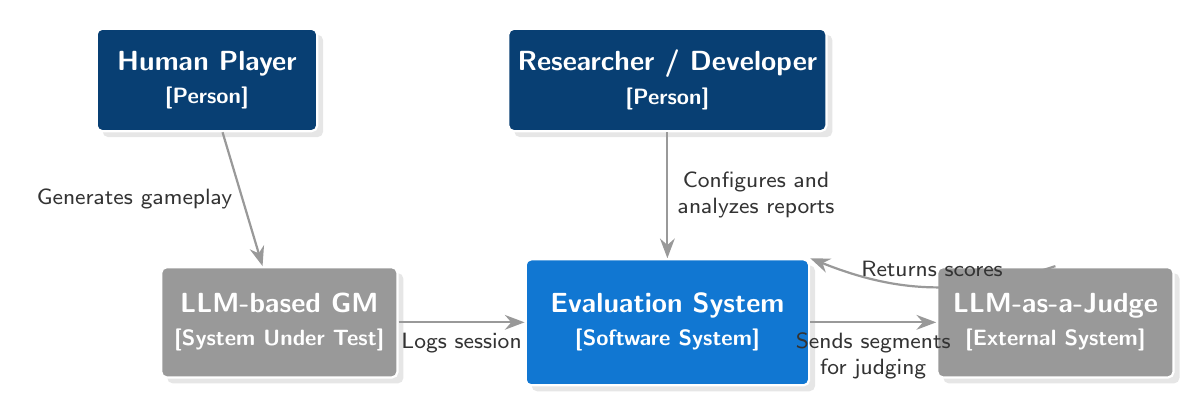
\begin{tikzpicture}[node distance=2.0cm and 2.4cm]
    % Actors
    \node[c4person] (researcher) {Researcher / Developer \\ \footnotesize [Person]};
    \node[c4person, left=of researcher] (player) {Human Player \\ \footnotesize [Person]};
    % Main System
    \node[c4system, below=1.6cm of researcher] (evalsys) {Evaluation System \\ \footnotesize [Software System]};
    % External Systems
    \node[c4external, left=1.6cm of evalsys] (gm) {LLM-based GM \\ \footnotesize [System Under Test]};
    \node[c4external, right=1.6cm of evalsys] (judge) {LLM-as-a-Judge \\ \footnotesize [External System]};
    % Relationships
    \draw[c4rel] (researcher) -- node[right] {Configures and \\ analyzes reports} (evalsys);
    \draw[c4rel] (player) -- node[left] {Generates gameplay} (gm);
    \draw[c4rel] (gm) -- node[below] {Logs session} (evalsys);
    \draw[c4rel] (evalsys) -- node[below] {Sends segments \\ for judging} (judge);
    \draw[c4rel] (judge.north) to[bend left=20] node[above] {Returns scores} (evalsys.north east);
\end{tikzpicture}
\caption{C4 Level 1 diagram: context of the LLM evaluation protocol. Human players generate gameplay through an LLM-based GM; sessions are logged and processed by the Evaluation System, which delegates judging to an LLM-as-a-Judge and reports back to the researcher.}
\label{fig:c4-context}
\end{figure}

The relevant actors and systems are: \textit{(i)} \textbf{Human Players} interact with the GM, providing the actions and choices that generate raw gameplay data; \textit{(ii)} the \textbf{Researcher / Developer} is the primary beneficiary, who configures the evaluation (metrics and weights), selects sessions, and analyzes the final reports; \textit{(iii)} the \textbf{LLM-based GM} is the system under test, providing narrations, responses, and world events; \textit{(iv)} the \textbf{Evaluation System} (the protocol) receives structured logs, processes them, and coordinates the evaluation; and \textit{(v)} the \textbf{LLM-as-a-Judge} receives specific segments and judging criteria, returning scores and justifications.

\subsection{Inputs and Outputs}

The system's external inputs consist of registered gameplay sessions containing player actions, GM responses, interaction types, and metadata. In open-world scenarios, the logs must also distinguish between sessions, ensuring that state consistency is evaluated only within the correct context. Additionally, the system receives a configuration defining metrics, weights, and judging criteria.

The external outputs are the evaluation results, which include Likert-scale scores per metric, a weighted global score, and qualitative evaluation traces (justifications). These outputs enable the identification of specific performance dimensions, such as high narrative quality paired with low state consistency, and support the recognition of patterns like persona breaks or technical admissions.

\subsection{Beneficiaries and Value Scenarios}

The protocol produces value across three main profiles. \textbf{Researchers} can perform reproducible comparisons between different LLMs to observe how narrative quality and coherence vary. \textbf{Developers} can identify recurring integration issues, memory failures, or context-filtering problems. \textbf{Game Designers} can monitor whether the artificial GM maintains a consistent experience across combat, dialogue, and exploration.

% =============================================================================
\section{Logical Vision}
\label{sec:logical}

This section describes the logical organization of the system, defining the abstract functions required to transform recorded gameplay sessions into evaluation results. Following the C4 Model approach \cite{brown:2024} at Level~2, this view focuses on functional containers that remain independent of specific programming languages or file formats.

\subsection{Component Architecture and Responsibilities}

The logical architecture decouples data collection, processing, judgment, and aggregation to ensure that the process is both reproducible and extensible. Figure~\ref{fig:c4-containers} shows the container-level decomposition.

\begin{figure}[ht]
\centering
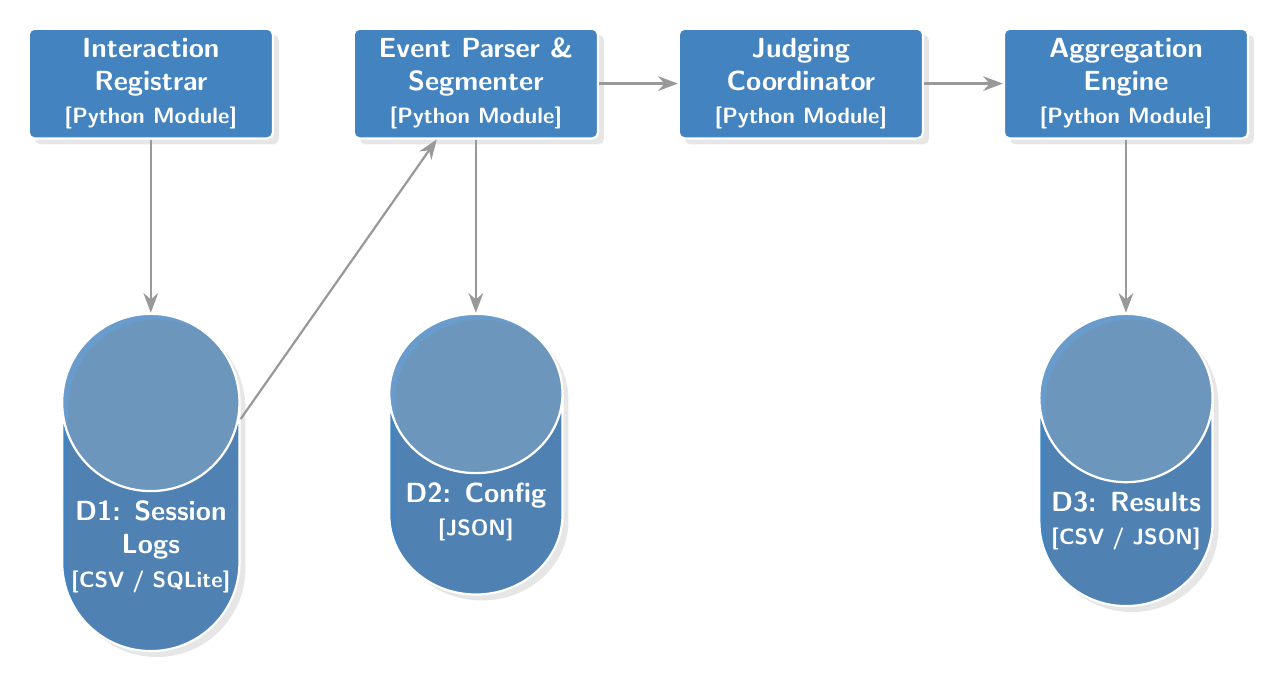
\begin{tikzpicture}[node distance=1.0cm and 1.0cm]
    % Internal Containers
    \node[c4container] (registrar) {Interaction \\ Registrar \\ \footnotesize [Python Module]};
    \node[c4container, right=of registrar] (parser) {Event Parser \& \\ Segmenter \\ \footnotesize [Python Module]};
    \node[c4container, right=of parser] (judgecoor) {Judging \\ Coordinator \\ \footnotesize [Python Module]};
    \node[c4container, right=of judgecoor] (aggregator) {Aggregation \\ Engine \\ \footnotesize [Python Module]};
    % Databases
    \node[c4db, below=2.2cm of registrar] (d1) {D1: Session \\ Logs \\ \footnotesize [CSV / SQLite]};
    \node[c4db, below=2.2cm of parser] (d2) {D2: Config \\ \footnotesize [JSON]};
    \node[c4db, below=2.2cm of aggregator] (d3) {D3: Results \\ \footnotesize [CSV / JSON]};
    % Flows
    \draw[c4rel] (registrar) -- (d1);
    \draw[c4rel] (d1) -- (parser);
    \draw[c4rel] (parser) -- (d2);
    \draw[c4rel] (parser) -- (judgecoor);
    \draw[c4rel] (judgecoor) -- (aggregator);
    \draw[c4rel] (aggregator) -- (d3);
\end{tikzpicture}
\caption{C4 Level 2 diagram: containers of the evaluation system and data persistence. Four Python modules form the pipeline; three persistence stores hold session logs, configuration, and final results.}
\label{fig:c4-containers}
\end{figure}

The system is composed of four primary logical functions:

\begin{itemize}[leftmargin=2.4em,itemsep=2pt]
  \item \textbf{Interaction Registration:} transforms the RPG session into a structured sequence of events. Each event preserves the relationship between the player's input and the system's response, along with metadata that enables the reconstruction of the interaction context.
  \item \textbf{Event Analysis and Normalization:} reads the session records, identifies relevant events, and discards or reduces data that do not contribute directly to the evaluation. A sub-function of segment selection picks the snippets suitable for each metric (action-response pairs for coherence, narrative blocks for quality, multi-turn sequences for state consistency).
  \item \textbf{Judgment by LLM:} applies evaluation criteria to each selected segment. The evaluator receives a segment, a specific metric, and scoring instructions, producing a Likert score and a justification. Separating prompts by metric makes the process auditable and reduces cross-criteria contamination.
  \item \textbf{Aggregation:} combines individual scores into metric-specific results and a weighted global score.
\end{itemize}

\subsection{Data Flow and Logic}

The logic of the system is entirely metric-driven. The GS1, GS3, and GS6 metrics concentrate most of the score because they represent the core pillars of narrative quality, action-to-narration coherence, and state consistency. Metrics GS4, GS5, and QC1 serve as complementary measurements for internal calibration, mechanical efficiency, and feedback quality. When open-world exploration is active, scenario-specific metrics are incorporated and weights are redistributed accordingly.

% =============================================================================
\section{Physical Vision}
\label{sec:physical}

This section explains how the system was effectively constructed, detailing languages, modules, files, data formats, persistence layers, LLM backends, and generated artifacts. It describes how the abstract protocol was materialized into an executable evaluation tool.

\subsection{Implementation Overview}

The system is implemented in Python, with the \texttt{rpg\_judge.py} module serving as the core component responsible for automatic evaluation. The module accepts either a single CSV session file or a directory for batch processing. Upon execution, it produces two primary artifacts: \texttt{rpg\_judge\_resultados.csv}, a file containing one record per session that enables individual inspection; and \texttt{rpg\_judge\_agregado.json}, a file with aggregated statistics per model that facilitates comparative analysis.

\subsection{Persistence and Data Formats}

The physical persistence strategy uses a three-layer approach to ensure narrative consistency and traceability. \textbf{Session logs (CSV)} record player inputs, system responses, interaction types, timestamps, token consumption, and response times; since April 2026, input and response fields are recorded without truncation up to 2000 characters, ensuring that full narratives are available for judgment. \textbf{Journey state (JSON)} maintains the current status of the player's progress and narrative milestones. \textbf{Long-term memory (SQLite)} stores NPC dialogue history and environmental facts mapped to specific coordinates in the open world. This layered architecture allows the system to re-inject relevant information back into the LLM's context, rather than relying solely on the model's internal memory window.

\subsection{Scenario Implementations}

The game implementation includes three distinct interaction scenarios that provide data for the evaluation protocol. \textbf{Scenario A (Combat)} executes a multi-step pipeline per turn, including ASCII HUD presentation, LLM-based creativity (0--1) and efficiency (0--2) assessment, damage calculation, streaming narration, and status-effect management (bleeding, poison, paralysis). \textbf{Scenario B (Dialogue)} distributes long-term memory functions between post-battle interactions and open-world conversations through a unified \texttt{NPC.falar()} mechanism, preserving the dialogue dimensions originally targeted at a separate scenario. \textbf{Scenario C (Open World)} manages exploration across an $(x,y,z)$ coordinate grid; biomes are determined by Euclidean distance from the origin (e.g., forests, plains, ruins), and each location is persisted with a procedurally generated name, an LLM-generated description, and a history of environmental modifications. Table~\ref{tab:env-modifications} lists the modification types detected.

\begin{table}[ht]
\centering
\caption{Environmental modifications persisted by coordinate in Scenario C.}
\label{tab:env-modifications}
\begin{tabular}{ll}
\toprule
\textbf{Type} & \textbf{Detected keywords} \\
\midrule
Fire        & fireball, blaze, flames \\
Cut         & I cut the tree, axe, fells \\
Magic       & I conjure, I cast, arcane bolt \\
Excavation  & I dig, excavate, pickaxe \\
Construction & I build, raise, barricade \\
Ice         & I freeze, snow, freeze \\
Explosion   & I blast, blast \\
Water       & I flood, flood \\
\bottomrule
\end{tabular}
\end{table}

\subsection{Model Integration and Backend}

The architecture supports a model-agnostic requirement (R4) through a unified interface (\texttt{llm\_backend.py}) and a runtime configuration file (\texttt{llm\_config.py}). Supported backends include Ollama (local), LM~Studio~0.4.11 (local API), and optional remote APIs. The backend and model selection are read at runtime for each call without caching, allowing model swapping without system restarts. The system also incorporates specific parsing to handle reasoning models by using regular expressions to filter out internal \texttt{<think>...</think>} blocks; this ensures that internal reasoning tokens do not appear in the player's narration or corrupt the evaluation JSON.

% =============================================================================
\section{Delimitation, Configuration, Extensibility, and Reproducibility}
\label{sec:delimitation}

This section explicitly states the scientific and technical limits of the system, indicating what was effectively evaluated, what is configurable, and how the protocol ensures a valid scientific study.

\subsection{Scope and Delimitation}

The primary delimitation of this study is that the evaluation is performed on structured gameplay logs rather than through automated gameplay or autonomous simulation. The evidence produced is based on 10 sessions involving 3 human players, with sessions ranging from 30 to 60 rounds each. This decision prioritizes the analysis of genuine interactions with variations in player styles, but findings are limited by the number of sessions, the specific scenarios executed, and the interaction styles captured within the logs. The protocol evaluates behavior already recorded, rather than real-time system performance.

\subsection{System Configuration}

The system is designed to be highly configurable across multiple layers to support comparative research. \textbf{Metric weights} are adjustable, defining how individual judgments are transformed into a weighted global score. \textbf{Model selection} (generative model and evaluator model) is independent. \textbf{Dynamic backends} are configurable at runtime, allowing the researcher to switch models without system restarts. \textbf{Batch processing} enables the evaluation of a single isolated session or a large set of sessions in batch mode.

\subsection{Extensibility}

The modular architecture allows the protocol to be adapted to other interactive LLM-based domains. Because the evaluation is based on structured logs and weighted aggregation, \textit{new metrics} can be added by defining their criteria and analysis units. The structure is applicable to \textit{narrative assistants}, \textit{long-term conversational agents}, and \textit{educational role-play simulations}. A constraint is that transferring to a new domain requires a review of the metrics, since dimensions suited for RPGs (e.g., state consistency) may not be sufficient for all interactive systems.

\subsection{Reproducibility and Scientific Validity}

Reproducibility is achieved through rigorous technical and methodological decisions: structured logs, fixed and versioned prompts, and deterministic configurations (fixed seed, temperature, top-p) ensure consistent results across trials, and every call to the model logs its specific parameters for later audit. The study acknowledges that LLM-as-a-judge is not ground truth: it provides a correlated estimate, not an equivalent to human judgment. The protocol explicitly recognizes potential evaluator bias and circularity (when the same model generates and judges); the latter is mitigated by using \texttt{qwen2.5:7b-instruct} as judge while other models act as generators in formal evaluations. Although three human players conducted the sessions, this trial did not include a formal subjective immersion scale, which remains a direction for future validation.

% =============================================================================
\section{Results}
\label{sec:results}

This section summarizes the preliminary evaluation results conducted over a reference session (69 inputs, 34 narrations, 5 questionnaire responses) and additional sessions with distinct models. Table~\ref{tab:results} reports the average scores obtained across the three dominant metrics and the aggregated global score.

\begin{table}[ht]
\centering
\caption{Experimental results per model (Likert scale 1--5). $n$ = number of evaluated sessions; \textbf{bold} = best per column.}
\label{tab:results}
\small
\begin{tabular}{lccccc}
\toprule
\textbf{Model} & $n$ & \textbf{GS1} & \textbf{GS3} & \textbf{GS6} & \textbf{Global} \\
\midrule
\texttt{qwen2.5:7b-instruct}                           & 1 & \textbf{4.79} & \textbf{5.00} & 2.94          & \textbf{3.87} \\
\texttt{gemma4:e2b}~$^{\dagger}$ \cite{deepmind:gemma4:2026} & 1 & 4.54          & 4.84          & \textbf{2.97} & 3.70          \\
\texttt{qwen2.5:1.5b}                                  & 7 & 3.21          & 4.88          & 2.21          & 3.14          \\
\texttt{qwen2.5:0.5b}                                  & 1 & 3.34          & 3.52          & 2.04          & 3.07          \\
\bottomrule
\end{tabular}
\\[2pt]
{\footnotesize $^{\dagger}$ Score obtained after adapting the parser of \texttt{rpg\_judge.py} to reasoning models (stripping \texttt{<think>} blocks and locating the last balanced JSON), achieving a 100\% parse success rate (196/196 calls). Before the adaptation, the same model recorded Global $\approx 1.9$ due to extraction failures: a result of integration engineering, not of model capacity.}
\end{table}

\subsection{Quantitative Analysis}

For interpreting the Likert scale (1--5), scores near 4.0 indicate consistent narrative performance, while values below 3.0 reveal frequent inconsistencies (turn-based contradictions, incorrectly narrated actions, or generic descriptions). Following the threshold adopted in RPGBench \cite{yu:2025}, a score of $\geq 3.0$ marks the baseline for a GM LLM's utility.

\textbf{The \texttt{qwen2.5:7b-instruct} and \texttt{gemma4:e2b} models stand out as the only two to exceed the approval threshold ($\geq 3.0$) in all dominant metrics, with surprisingly close profiles:} the 7B-instruct wins on GS1/GS3, while \texttt{gemma4:e2b} (effective 2B) wins on GS6, evidence that architecture and training regime can compensate for parameter count in maintaining state consistency. The smaller variants of the Qwen2.5 family (1.5B and 0.5B) sit just above the threshold; \texttt{qwen2.5:1.5b} exhibited high variance across sessions (Global $\in [1.95;~3.72]$, $\sigma=0.81$, $n=7$), indicating sensitivity to injected history and player style. \textbf{GS6 (state consistency) remains the primary bottleneck:} even the best model lands at 2.97, on the floor of the threshold, and long-term coherence continues to be the hard limit of open-weight sub-10B models. GS3 saturates near 5.00 in models $\geq 1.5$B, indicating that simple actions are faithfully narrated. Although limited in scale ($n=10$ sessions, four models, three scenarios), these results are sufficient to demonstrate the \textit{discriminative capacity} of the proposed protocol: the metrics separate models with distinct profiles in a reproducible manner and expose the consistency gap as the priority direction for future versions.

\subsection{Observed Failure Modes}

Qualitative analysis revealed five systematic patterns of failure, more frequent in models with fewer than 7B parameters:

\begin{enumerate}[label=(\roman*),leftmargin=2.4em,itemsep=2pt]
  \item \textbf{Internal variable leakage:} \texttt{qwen2.5:0.5b} added an unsolicited field to the output JSON (\texttt{"needs\_engaging\_context"});
  \item \textbf{History-contaminated hallucination:} an incorrect player name (\textit{``Silvano''}) propagated across sessions and models (\texttt{qwen2.5:1.5b} and \texttt{gemma4:e2b});
  \item \textbf{Persona breaks with meta-apologies:} \texttt{qwen2.5:1.5b} answered as a technical assistant (\textit{``I apologize for the previous confusion...''}) instead of staying in character;
  \item \textbf{Log prefix leakage:} \texttt{gemma4:e2b} literally reproduced structural labels (\texttt{Yara:}, \texttt{Fe:}) from the history;
  \item \textbf{Admission of technical limitations:} the model justified missing information by stating \textit{``I don't have the capacity''}, instead of building a narrative barrier.
\end{enumerate}

Regarding timing, failures emerged as early as turn~0 when the injected history contained errors from previous tests, and between turns~1 and~4 in NPC dialogues, due to context accumulation exceeding the attention window of small models for negative instructions (\textit{``do not break persona''}).

% =============================================================================
\section{Conclusion}

This work presented a reproducible evaluation protocol for LLM-based Game Masters, materialized in the \texttt{rpg\_judge.py} module. The protocol operates over an autonomous GM system featuring three distinct scenarios (combat, dialogue, and open-world exploration) executing entirely on local LLMs. The three-layer persistence architecture (SQLite, JSON, CSV) proved effective in supporting narrative consistency, providing a robust framework for metrics comparable to those established in RPGBench \cite{yu:2025}.

The value of this system lies in offering an auditable and extensible process for the preliminary and comparative evaluation of interactive agents. \textbf{The proposed protocol is not restricted to RPGs:} its structure of structured logs, weighted metrics, and LLM-as-a-judge is directly applicable to other stateful interactive systems, including narrative assistants, long-duration conversational agents, and educational role-play simulations.

As future work, we intend: (1) \textit{human validation}, conducting studies with human evaluators to correlate automatic metrics with subjective perceptions of quality and immersion; (2) \textit{multi-judge consensus}, implementing multiple judge models to reduce circularity and increase robustness; (3) \textit{lexical diversity}, refining narrative metrics with TTR and MTLD analysis \cite{reviriego:2024}; (4) \textit{long-term semantic memory}, integrating FAISS vector databases for semantic retrieval; and (5) \textit{open-world expansion}, extending Scenario~C with complex dialogue encounters in the procedurally generated world. By establishing the protocol and the conceptual and logical visions before detailing the physical implementation, this work provides a practical and extensible framework for evaluating interactive, stateful LLM-based systems.

\textbf{Acknowledgments.} [OMITTED FOR ANONYMOUS REVIEW]

\bibliographystyle{sbc}
\bibliography{Referencias/referencias}

\end{document}
